\documentclass[a4paper]{article}

%% Language and font encodings
\usepackage[french]{babel}
\usepackage[utf8x]{inputenc}
\usepackage[T1]{fontenc}

%% Sets page size and margins
\usepackage[a4paper,top=3cm,bottom=3cm,left=2cm,right=2cm,marginparwidth=2cm]{geometry}
%% Useful packages
\usepackage{amsmath}
\usepackage{graphicx}
\usepackage[colorinlistoftodos]{todonotes}
\usepackage[colorlinks=true, allcolors=black]{hyperref}
\usepackage{fourier-orns}
\usepackage{titlesec}
\usepackage{fancyhdr}
\usepackage{fancyvrb}
%\renewcommand{\thefootnote}{\*}
\pagestyle{fancy} 
\setcounter{tocdepth}{5}

%% Tikz stuff
\usepackage{tikz}
\usetikzlibrary{calc, arrows}
\tikzstyle{incolore} = [rectangle, rounded corners, draw=black, minimum height=1cm, minimum width=3cm, text width=3cm, text centered]

\usepackage{libertine}
\newcommand{\hsp}{\hspace{20pt}}
\newcommand{\HRule}{\rule{\linewidth}{0.5mm}}

\renewcommand{\headrulewidth}{1pt}
\fancyhead[C]{}
\fancyhead[L]{}
\fancyhead[R]{\footnotesize{\scshape Introduction aux bases de données}}

\renewcommand{\footrulewidth}{1pt}
\fancyfoot[C]{}
\fancyhead[L]{}
\fancyfoot[R]{\thepage}

\definecolor{Zgris}{rgb}{0.87,0.85,0.85}

\usepackage{eso-pic,graphicx}
\usepackage{xcolor}
\newcommand{\bgimg}[1]{
\AddToShipoutPicture
    {
        \put(\LenToUnit{0 cm},\LenToUnit{0 cm})
        {
            \includegraphics[width=\paperwidth,height=\paperheight]{#1}
        }
    }
}
\begin{document}




%%\bgimg{Image_15.jpg}

















\begin{titlepage}
    \begin{sffamily}
        \begin{center}

            
\includegraphics[width=5cm]{images/LogoHenallux.PNG}~\\[1.5cm]
            \textsc{\Large Travail d'évaluation}\\[1.5cm]

            \HRule \\[0.4cm]
            { \huge \bfseries Énoncé et schéma conceptuel\\[0.4cm] }
            \HRule \\[2cm]

            \begin{minipage}{0.4\textwidth}
                \begin{flushleft} \large
                    Roumache Grégoire\\
                    Sécurité des systèmes\\
                    Première année, groupe H \\
                \end{flushleft}
            \end{minipage}
            \begin{minipage}{0.55\textwidth}
            \begin{flushright} \large
                Introduction aux bases de données\\
                Hénallux\\
                Année académique 2019-2020\\
            \end{flushright}
            \end{minipage}
            \vfill

            {\large 22 Avril 2020}
        \end{center}
    \end{sffamily}
\end{titlepage}







\let\cleardoublepage\clearpage















\section{Énoncé}





Une compagnie pétrolière a besoin d'une base de données qui enregistre plusieurs éléments allant de l'extraction du pétrole jusqu'au consommateur.

La production commence avec les puits qui sont référencés par un id et qui sont liés à une raffinerie par une pipeline. Le système doit enregistrer la profondeur du puit ainsi que les réserves de pétrole qu'il contient et sa production journalière.

Les raffineries sont elles aussi référencées par un id et le système doit connaître leur production journalière et le nombre d'employés, ainsi que la production maximale possible de la raffinerie.

Le camion-citerne est un élément très important pour une entreprise pétrolière. Il sert à faire la liaison entre une raffinerie et des stations-services. En effet, il se remplit dans une raffinerie et ravitaille les stations-services en essence. On identifie les camions-citernes grâce à leur immatriculation. On veut connaître à tout instant le niveau d'essence dans le réservoir du camion-citerne et son niveau de carburant (carburant que le camion consomme).

Comme pour les raffineries, on veut connaître le nombre d'employés qui travaillent dans chaque station-service. Les stations services sont identifiées par un id et on veut connaître leur capacité, c-à-d la quantité d'essence qu'elles peuvent contenir au maximum. Le système doit aussi enregistrer leur réserve qui est la quantité d'essence disponible à un moment donné.















\section{Schéma conceptuel}





\begin{center}
    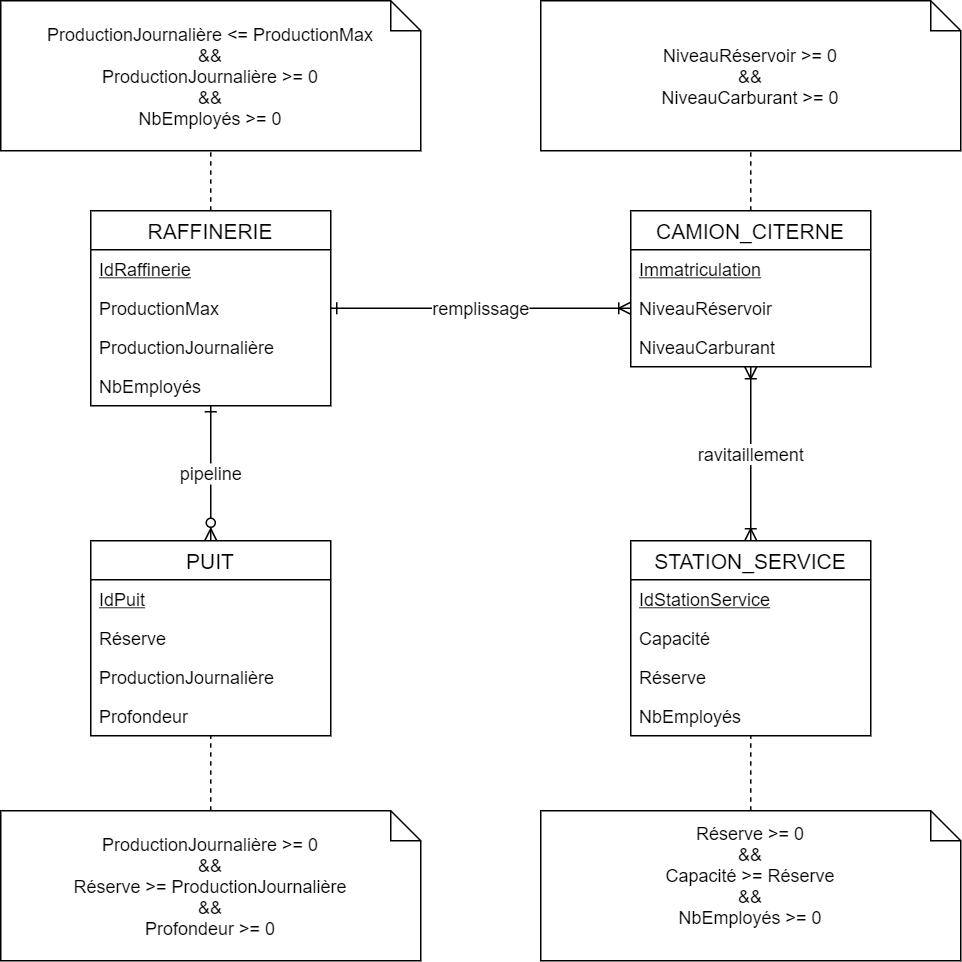
\includegraphics[width=0.85\textwidth]{images/RoumacheGregoire_ERD.png}
\end{center}



















\end{document}
